\documentclass[10pt,landscape, fleqn]{article}
\usepackage{multicol}
\usepackage{mathtools}
\usepackage{calc}
\usepackage{ifthen}
\usepackage[landscape]{geometry}
\usepackage{hyperref}
\usepackage[calcwidth]{titlesec}
\usepackage{enumitem}

\ifthenelse{\lengthtest { \paperwidth = 11in}}
{ \geometry{top=.5in,left=.5in,right=.5in,bottom=.5in} }
{\ifthenelse{ \lengthtest{ \paperwidth = 297mm}}
	{\geometry{top=1cm,left=1cm,right=1cm,bottom=1cm} }
	{\geometry{top=1cm,left=1cm,right=1cm,bottom=1cm} }
}

% Do not indent equations
\setlength{\mathindent}{0pt}

% Turn off header and footer
\pagestyle{empty}


% Redefine section commands to use less space
%\makeatletter
%\renewcommand{\section}{\@startsection{section}{1}{0mm}% 
%	{-1ex plus -.5ex minus -.2ex}%
%	{0.5ex plus .2ex}%x
%	{\normalfont\large\bfseries}
%	}
\titleformat{\section} {\normalfont\large\bfseries}{\thesection}{1em}{}[{\titlerule[1.5pt]}]
\titlespacing{\section}{0.0em}{.5ex}{.5ex} % {left}{before}{after}[right]
%\renewcommand{\subsection}{\@startsection{subsection}{2}{0mm}%
%	{-1explus -.5ex minus -.2ex}%
%	{0.5ex plus .2ex}%
%	{\normalfont\normalsize\bfseries}}
\titleformat{\subsection}{\normalfont\normalsize\bfseries}{\thesection}{0.5em}{}[\vspace{-1em}\rule{\titlewidth}{0.3pt}]
\titlespacing{\subsection}{0.0em}{0ex}{0ex} % {left}{before}{after}[right]
% \renewcommand{\subsubsection}{\@startsection{subsubsection}{3}{0mm}%
%	{-1ex plus -.5ex minus -.2ex}%
%	{1ex plus .2ex}% 
%	{\normalfont\small\bfseries}}
%\makeatother
\titleformat{\subsubsection} {\normalfont\small\bfseries}{\thesection}{0.5em}{}
\titlespacing{\subsubsection}{0.0em}{0ex}{0ex} % {left}{before}{after}[right]

\setlist[itemize]{leftmargin=*}
\setlist[enumerate]{leftmargin=*}

% Define BibTeX command
\def\BibTeX{{\rm B\kern-.05em{\sc i\kern-.025em b}\kern-.08em
		T\kern-.1667em\lower.7ex\hbox{E}\kern-.125emX}}

% Don't print section numbers
\setcounter{secnumdepth}{0}


\setlength{\parindent}{0pt}
\setlength{\parskip}{1pt plus 0.5ex}


% -----------------------------------------------------------------------

\begin{document}
	\raggedright
	\footnotesize
		
	\begin{center}
		\Large{\textbf{Applied Statistics Cheatsheet}} \\
	\end{center}
	\begin{multicols}{3}
		% multicol parameters
		% These lengths are set only within the two main columns
		%\setlength{\columnseprule}{0.25pt}
		\setlength{\premulticols}{1pt}
		\setlength{\postmulticols}{1pt}
		\setlength{\multicolsep}{1pt}
		\setlength{\columnsep}{2pt}
		\section{Statistical Inference}
			An \textbf{inference} is a conclusion that patterns in the data are present in some broader context.
			A \text{statistical inference} is an inference justified by a probability model linking the data to the broader context.
			\begin{itemize}
				\item \textbf{Observational Study}: The group status of the subjects is established beyond the control of the investigator.
				\item \textbf{Randomized Experiment}: the investigator controls the assignment of experimental units to groups and uses a chance mechanism (like the flip of a coin) to make the assignment
			\end{itemize}
			\subsection{Causal Inference}
				Statistical inferences of cause-and-effect relationships can be drawn 	from randomized experiments, but not from observational studies.
				\subsubsection{Counfounding Variables} 
				A confounding variable is \textbf{related both to group membership and to the outcome}. Its presence makes it hard to establish the outcome as being a direct consequence of group membership
			\subsection{Inference to populations}
				Inferences to populations can be drawn from random sampling	studies, but not otherwise.\par 
				Random sampling ensures that all subpopulations are represented in the sample in roughly the same mix as in the overall population. Again,
			\subsection{Simple Random Sample}
				A simple random sample of size n from a population is a subset of the 	population consisting of n members selected in such a way that every subset of size n is afforded the same chance of being selected.
			
		\section{Simple Linear Regression}
			$\mu\{Y|X\} = \beta_0 + \beta_1X$
			\subsection{Model Assumption}
				\begin{enumerate}
					\item Linearity
					\item Normality: ${Y|X} \sim Normal$
					\item Constant Variance: $\sigma(Y|X)=\sigma$
					\item Independence
				\end{enumerate}
			\subsection{Least Square Method}
				Minimize $ Q = \sum(Y_i - b_0 - b_1X_i)^2 = \sum(Y_i - \hat{Y_i})^2 $
				\[b_1 = \frac{\sum_{1}^{n}(X_i-\bar{X})(Y_i-\bar{Y}))}{\sum_{i=1}^{n}(X_i-\bar{X})^2} \]
				\[b_0 = \bar{Y} - b1\bar{X} \]
				\[ \hat{\sigma}=\sqrt{\frac{\sum_{j=1}^{n}(Y_i-\hat{Y_i})^2}{n-2}} \]
			\subsection{Sampling Distribution}
				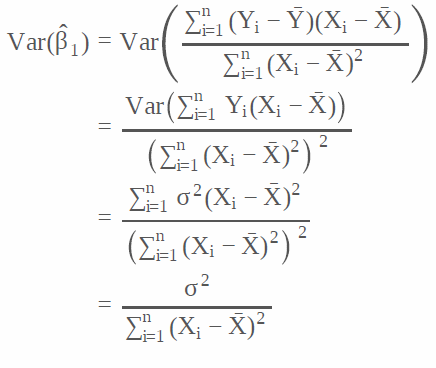
\includegraphics[width=0.6\linewidth]{slr1}
				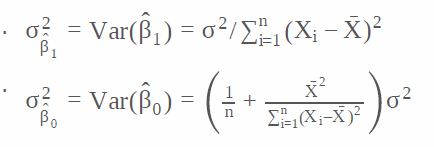
\includegraphics[width=0.7\linewidth]{slr2}
				\[ SD(b_1) = \hat{\sigma}\sqrt{\frac{1}{(n-1)\sigma_x^2}} \]
				\[ SD(b_0) = \hat{\sigma}\sqrt{\frac{1}{n} + \frac{\bar{X}^2}{(n-1)\sigma_x^2}} \]
				\[ \frac{b_1-\beta_1}{SE(B_1)} \sim t(n-2) \ \ \frac{b_0-\beta_0}{SE(B_0)} \sim t(n-2) \]
			\subsection{Matrix Form}
				$ Y = X\beta + \epsilon $
				\[ Y = \left[ 
						\begin{array}{c}
							Y_1\\ Y_2 \\ . \\ Y_n
						\end{array}
						\right]  = \left[
						\begin{array}{c c}
							1 & X_1 \\
							1 & X_2 \\
							. & . \\
							1 & X_n \\
						\end{array}
						\right]\left[
							\begin{array}{c}
								\beta_0\\
								\beta_1
							\end{array}
						\right] + \left[
							\begin{array}{c}
								\epsilon_1 \\
								\epsilon_2 \\
								. \\
								\epsilon_n
							\end{array}
						\right]
				\]

				\[\Psi = (Y-X\beta)^T(Y-X\beta) \]
				\[ \hat{\beta} = (X^TX)^{-1}X^TY \]
			\subsection{Confidence Intervals}
				$ SD(\mu(Y|X_0)) = \hat{\sigma}\sqrt{\frac{1}{n} + \frac{(X_0-\bar{X})^2}{(n-1)\sigma_x^2}} $
				\[ \mbox{standardized } \mu(Y|X_0) \sim t(n-2)\]
			\subsection{Prediction Interval}
				$ SD(Y|X_0) = \hat{\sigma}\sqrt{1+\frac{1}{n} + \frac{(X_0-\bar{X})^2}{(n-1)\sigma_x^2}} $
				\[ \mbox{standardized } Y|X_0 \sim t(n-2)\]
			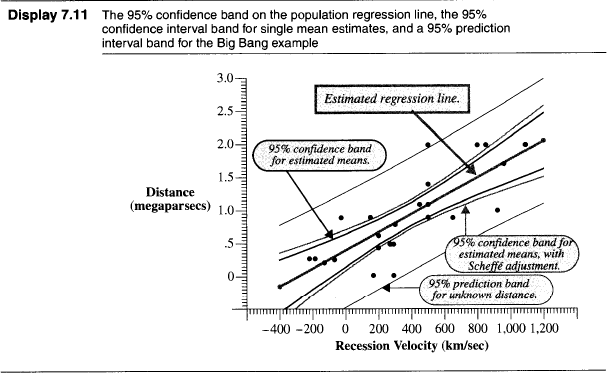
\includegraphics[width=0.95\linewidth]{slr3}
			\subsection{R Squared}
				Total sum of squares(\textbf{SST}) = $\sum_{i=1}^{n}(Y_I-\bar{Y})^2$ \par 
				Regression sum of squares(\textbf{SSR}) = $\sum_{i=1}^{n}(\hat{Y_i}-\bar{Y})^2$ \par 
				Residual sum of squares(\textbf{SSE}) = $\sum_{i=1}^{n}(Y_i-\hat{Y_i})^2$
				\[ SST = SSR + SSE \]
				\[ R^2 = (\frac{SST-SSE}{SST})\% = (\frac{SSR}{SST})\% \]
				\[ MSE = \frac{SSE}{n-2} \]
			\subsection{Extra-Sums-of-Squares F-test}
				$H_0: \beta_1=0$
				\[F-stat = \frac{\left[ \frac{\mbox{extra sums of squares}}{\# \beta\mbox{ being tested}} \right]}{\hat{\sigma}^2\mbox{ from full model}} 
				        =\frac{\frac{SSR_{full}-SSR_{null}}{1}}{MSE}\]
				
		\section{Multiple Regression}
			\[\hat{\sigma}^2 = \frac{\sum(Y_i-\hat{Y_i})^2}{n-p} = \frac{SSE}{n-p} \]
			\[SD(b_j) = \sigma\sqrt{c_{ij}} \]
			\[\mbox{standardized } b_j \sim t(n-p) \]
			$c_{ij}$ is $j^{th}$ diagonal element of $(X^TX)^{-1}$ \par 
			\subsection{Linear Combination Of Coefficients}
				\[ H_0: c_0\beta_0 + c_1\beta_1 + ... + c_p\beta_p = 0 \]
				\[ H_A: c_0\beta_0 + c_1\beta_1 + ... + c_p\beta_p \neq 0 \]
				\[ est=c_0b_0 + c_1b_1 + ... + c_pb_p \]
				\[
					\begin{split}
						Var(est) &= c_0^2Var(b_0)^2 + .. + c_p^2Var(b_0) \\
								&  +2c_0c_1Cov(b_0, b_1)+...+c_{p-1}c_{p}Cov(b_{p-1},b_{p})  \\
						 &= \hat{\sigma}^2C(X^TX)^{-1}
					\end{split}
				\]
			\subsection{Extra-Sums-of-Squares F-test}
			$H_0: \beta_1=\beta_2=...=\beta_p=0$
			\[F-stat = \frac{\left[ \frac{\mbox{extra sums of squares}}{\#\mbox{ of }\beta\mbox{'s being tested}} \right]}{\hat{\sigma}^2\mbox{ from full model}} 
			=\frac{\frac{SSR_{full}-SSR_{reduce}}{df_{reduce}-df_full}}{MSE}\]
			\[ MSE = \frac{SSE}{n-p-1} \]
			\subsection{Adjusted $R^2$}
				Only for model comparison, not for model assessment.
				\[ \mbox{Adjusted } R^2 = \frac{\frac{SST}{n-1}-\frac{SSE}{n-p}}{\frac{SST}{n-1}} \]			
			\subsection{Leverage}
				Measure the distance between explanatory values and the mean of explanatory values. 
				\[ H = X(X^TX)^{-1}X \]
				\[ \mbox{For ith observation: } h_i = H_{ii}  = \frac{\partial \hat{Y_i}}{\partial Y_i}\] 
				$SD(residual_i) = \sigma\sqrt{1-h_i}$ , $\bar{h_i} = p/n$ \par 
				Cutoff: larger than $2p/n$ ($p: $ the number of parameters)
			\subsection{Studentized Residual}
				\[ studres_i = \frac{residual_i}{\hat{\sigma}\sqrt{1-h_i}} \]
				Roughly normal distributed. (Check absolute residual lager than 2)
			\subsection{Cook's Distance}
				\[ D_i = \sum_{j=1}^{n}\frac{(\hat{Y}_{j(i)}-\hat{Y_j})^2}{p\hat{\sigma}^2} 
				       = \frac{1}{p}(studres_i)^2(\frac{h_i}{1-h_i})\]
				$\hat{Y}_{j(i)}$ is the jth fitted value without case i in the dataset \par
				Cutoff: Larger than 1 $\rightarrow$ influential
			\subsection{Model Diagnosis}
				\begin{enumerate}
					\item Residual v.s. Fitted Value Plot:
						\begin{itemize}
							\item Pattern?
							\item Non-constant Variance?
							\item Influential Overservations?
						\end{itemize}
					\item QQ-Plot: Normality
					\item Cook's Distance and Leverage Plot
				\end{enumerate}
				
		\section{Weighted Regression}
			\[ var(Y_i|X) = \frac{\sigma^2}{w_i} \]
			\[ Q = \sum w_i(Y_i-\hat{Y_i})^2 \]
			\[ \hat{\beta} = (X^TWX)^{-1}X^TWY \]
			\[ W = \left[ 
				\begin{array}{cccc}
					w_1 & 0 & . & 0 \\
					0 & w_2 & 0 & 0 \\
					. & . & . & . \\
					0 & 0 & 0 & w_n
				\end{array}
				\right] \]
		
		\section{Ridge and Lasso Regression}
			$|\beta_j|$: L1-norm
			\[ \mbox{Lasso: } \sum_{i=1}^{n}(y_i- \hat{y_i})^2 + \lambda\sum_{j=1}^{p}|\beta_j| \]
			$(\beta_j)^2$: L2-norm
			\[ \mbox{Ridge: } \sum_{i=1}^{n}(y_i- \hat{y_i})^2 + \lambda\sum_{j=1}^{p}(\beta_j)^2 \]
			\begin{center}
				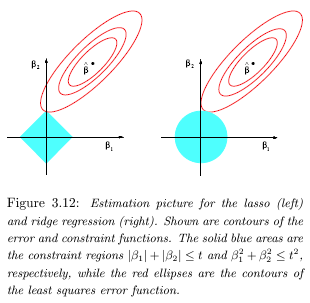
\includegraphics[width=0.7\linewidth]{regularization}
			\end{center}

		\section{Model Selection}
			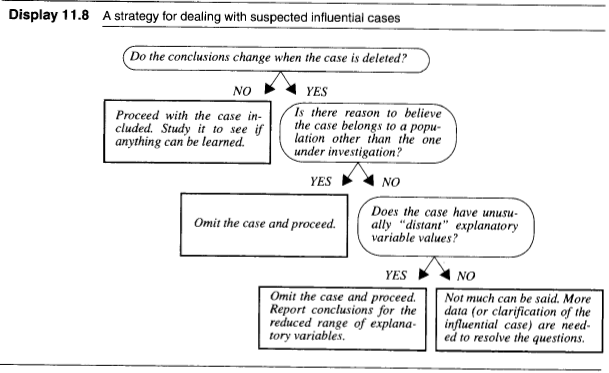
\includegraphics[width=0.95\linewidth]{mlr1}
			\subsection{Strategies}
				\subsubsection{Forward Selection}
					Start with the null model.
				\subsubsection{Backward Selection}
					Start with the full model.
				\subsubsection{Stepwise Selection}
					\begin{enumerate}
						\item Start with null model.
						\item Do on step of forward selection.
						\item Do one step of backward elimination.
						\item Repeat 2 and 3 until no explanatory variables can be added or removed.
					\end{enumerate}
				\subsubsection{Exhaustive Search Through All Subsets}
					Use the Cp statistics, $R^2$, Adjusted $R^2$, AIC and BIC.
			\subsection{Cp Statistic}
				The lower, the better.
				\[ Cp = p + (n-p)\frac{\hat{\sigma}^2 - \hat{\sigma}^2_{full}}{- \hat{\sigma}^2_{full}}\]
			\subsection{Akaike's Information Criteria(AIC)}
				The lower, the better.
				\[ AIC = 2p + n log(\hat{\sigma}^2) = 2p - 2log(L) \]
			\subsection{Bayesian Information Criteria(BIC)}
				The lower, the better.
				\[ BIC = p\cdot log(n) + n\cdot log(\hat{\sigma}^2) = p\cdot log(n) - 2log(L) \]
			\subsection{Model Validation}
				For a new data set, define \textbf{mean square prediction error} as:
				\[ MSPE = \frac{\sum_{i=1}^{k=1}(Y_i-\hat{Y}_i)^2}{k} \]
			\subsection{Cross Validation}
			
		\section{Serial Correlation}
			\subsection{First-Order Autoregression Model \{AR(1)\}}
				\[ Y_t = \beta_0 + \beta_1X_1 + ... + \beta_kX_k + \epsilon_t\]
				\[ \epsilon_t  = \alpha\epsilon_{t-1} + \psi_t \]
				\[ \psi_i \sim N(0, \sigma^2) \]
				Estimating $\alpha$: Use the correlation coefficient between subsequent ordinary regression residuals.
			\subsection{Partial Auto Correlation Function(PACF)}
				A plot of the partial autocorrelations against lags. \par 
				cutoff: $ [-\frac{2}{\sqrt{n}}, \frac{2}{\sqrt{n}}]$
			\subsection{Large-Sample Test}
				If one estimates the serial correlation coefficient from a series of n independent observations with constant variance, the estimate has an approx. normal distribution with mean 0 and standard deviation $\frac{1}{\sqrt{1}}$.
				
		\section{Variance Inflation Factor}
			\[ 
			\begin{split}
				\widehat{Var}(\hat{Bj}) &= \hat{\sigma^2}(X^TX)^{-1}_{j+1, j+1} \\
				    &= \frac{\hat{\sigma^2}}{(n-1)\widehat{Var}(X_j)}\frac{1}{1-R^2_j}
			\end{split}
			\]
			$R^2_j := R^2$ for the regression of $X_j$ on the other covariates.
			\[ VIF := \frac{1}{1-R^2_j} \]
			Cut-off rule of thumb: \par 
			$VIF(\hat{B_j}) > 5$ for high multicollinearity \par
			
		\section{Bootstrap}
			Assumption: 
			\textbf{Independence} between samples.
			\subsection{Non-parametric Bootstrap}
				Repeated re-sampling with replacement. \par 
				The number of different bootstrap samples is ${2n-1 \choose n}$ for sample size n. \par 
				Can obtain statistics(e.g. mean, standard deviation) of the estimator with only one set of samples. \par
			\subsection{Bootstrap Regression}
   			    Let $X$ be the explanatory variable, $Y$ be the responsive variable.
				\subsubsection{Case-based}
					\begin{enumerate}
						\item Re-sample based on $(X, Y)$ pairs. 
						\item Fit a regression model on the bootstrap sample.
						\item Repeat 1 and 2 several times.
					\end{enumerate}
					Problem: When $X$ is an indicator variable.
				\subsubsection{Residual-based}
					\begin{enumerate}
						\item Fit  regression model on the original sample. 
						\item Re-sample the residuals from 1 
						\item Add bootstrap residuals to $hat{Y}$ to form the new $Y'$.
						\item Fit a regression model on $Y'$ and $X$.
						\item Repeat 1-3 several times.
					\end{enumerate}
					Solve the problem of X being extremely skewed.
				\subsubsection{Bootstrap Confidence Interval}
					Useful when the distribution of estimator is skewed or not normal. \par
					Use quantiles of the bootstrap estimations as the boundary of the confidence interval.
			\subsection{Parametric Bootstrap}
				\begin{enumerate}
					\item A parametric model is fitted to the data (Often by maximum likelihood)
					\item Samples of random numbers are drawn from this fitted model
					\item Calculate the estimate/quantity of interest from these samples
					\item Repeat 2 and 3 many times as for other bootstrap methods
				\end{enumerate}
				Parametric bootstrap will be more accurate than non-parametric bootstrap if the parametric assumption is true, less accurate if false.
		\section{Natural Cubic Spline}
			\textit{splines} package in R
			\begin{enumerate}
				\item Dividing the range of $X$ into intervals.
				\item Inside each interval, a cubic polynomial model is fitted.
				\item At the interval split points(knots), the cubic polynomial are continuous and have continuous first and second derivatives.
			\end{enumerate}
			\begin{center}
				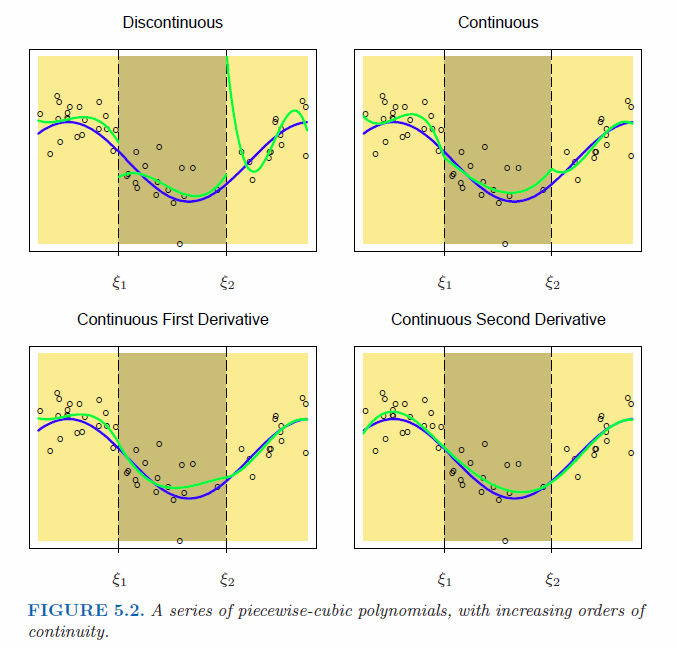
\includegraphics[width=0.95\linewidth]{Image}
			\end{center}
			R example: \par 
			$fit2<-lm(ozone\sim ns(temperature,knots=c(70,90)))$ \par
			$df = 2 + \mbox{\# of knots}$ \par 
			When to use natural cubic splines?
			\begin{enumerate}
				\item Smoothing.
				\item To model confounding variables.
				\item Higher order terms are required for $X$
			\end{enumerate}
		
		\section{Canonical Correlation Analysis (CCA)}
			CCA finds linear combinations in the two sets that have the largest possible correlations. \par
			R command: \textbf{cancof} 
			\subsection{Bartlett's Chi-square Test}
				How many pairs of canonical variables are significant?
				\[ V = -\left((n-1) - \frac{p+q+1}{2}\right)ln(k) \]
				n: number of obvservations \\
				p: number of X variables minus number times test applied \\
				q: number of Y variables minus number times test applied\\
				k:  $(1-r_t^2)(1-r^2_{t+1})...(1-r_T^2)$ \\
				$r_j^2$: the squared correlation between the jth pair of canonical variables. \\
				T: The totla number of canonical variables\\
				t: number of times test applied \\
				$V \sim \chi_{pq}^2$ under $H_0:$ the pair is significant.
				
		\section{Principle Component Analysis}
			\begin{center}
				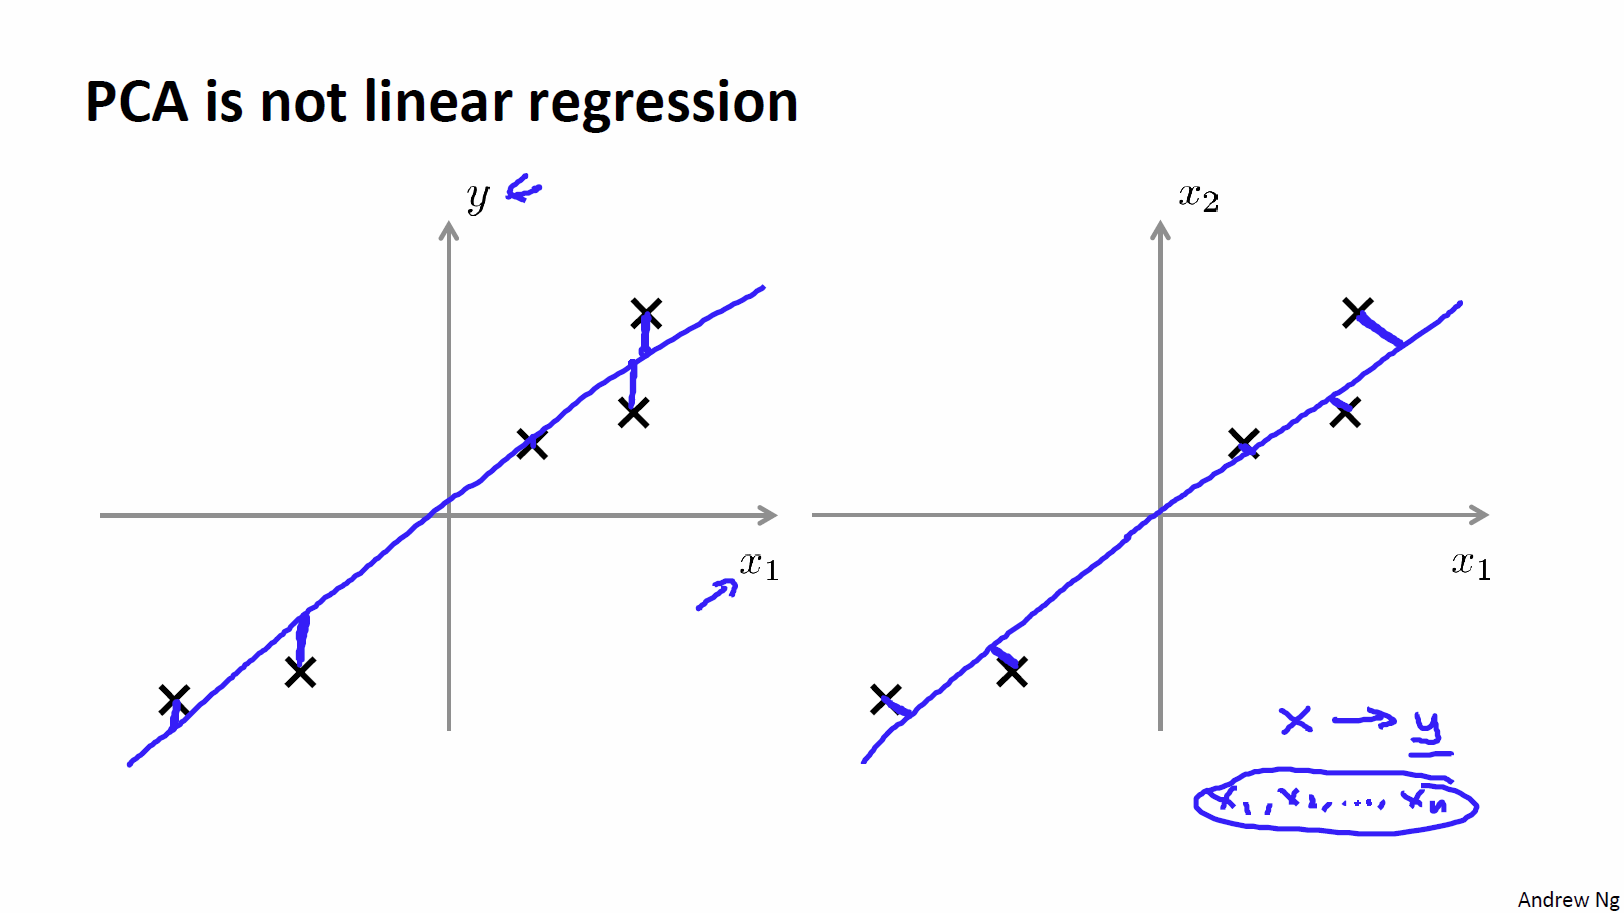
\includegraphics[width=0.95\linewidth]{pca1}
				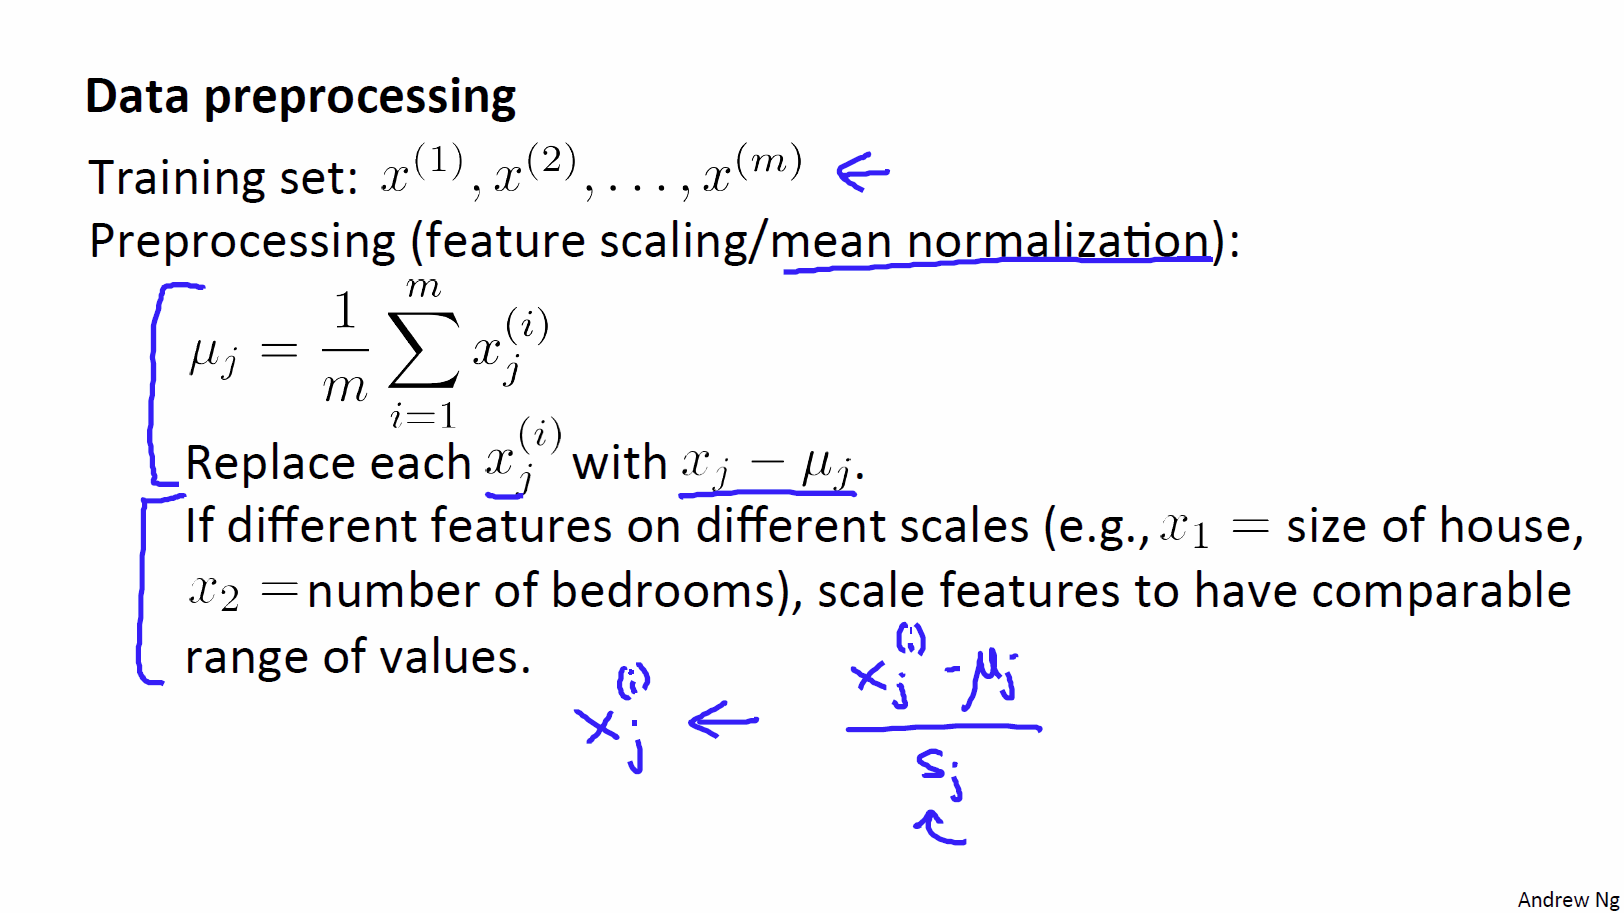
\includegraphics[width=0.95\linewidth]{pca2}
				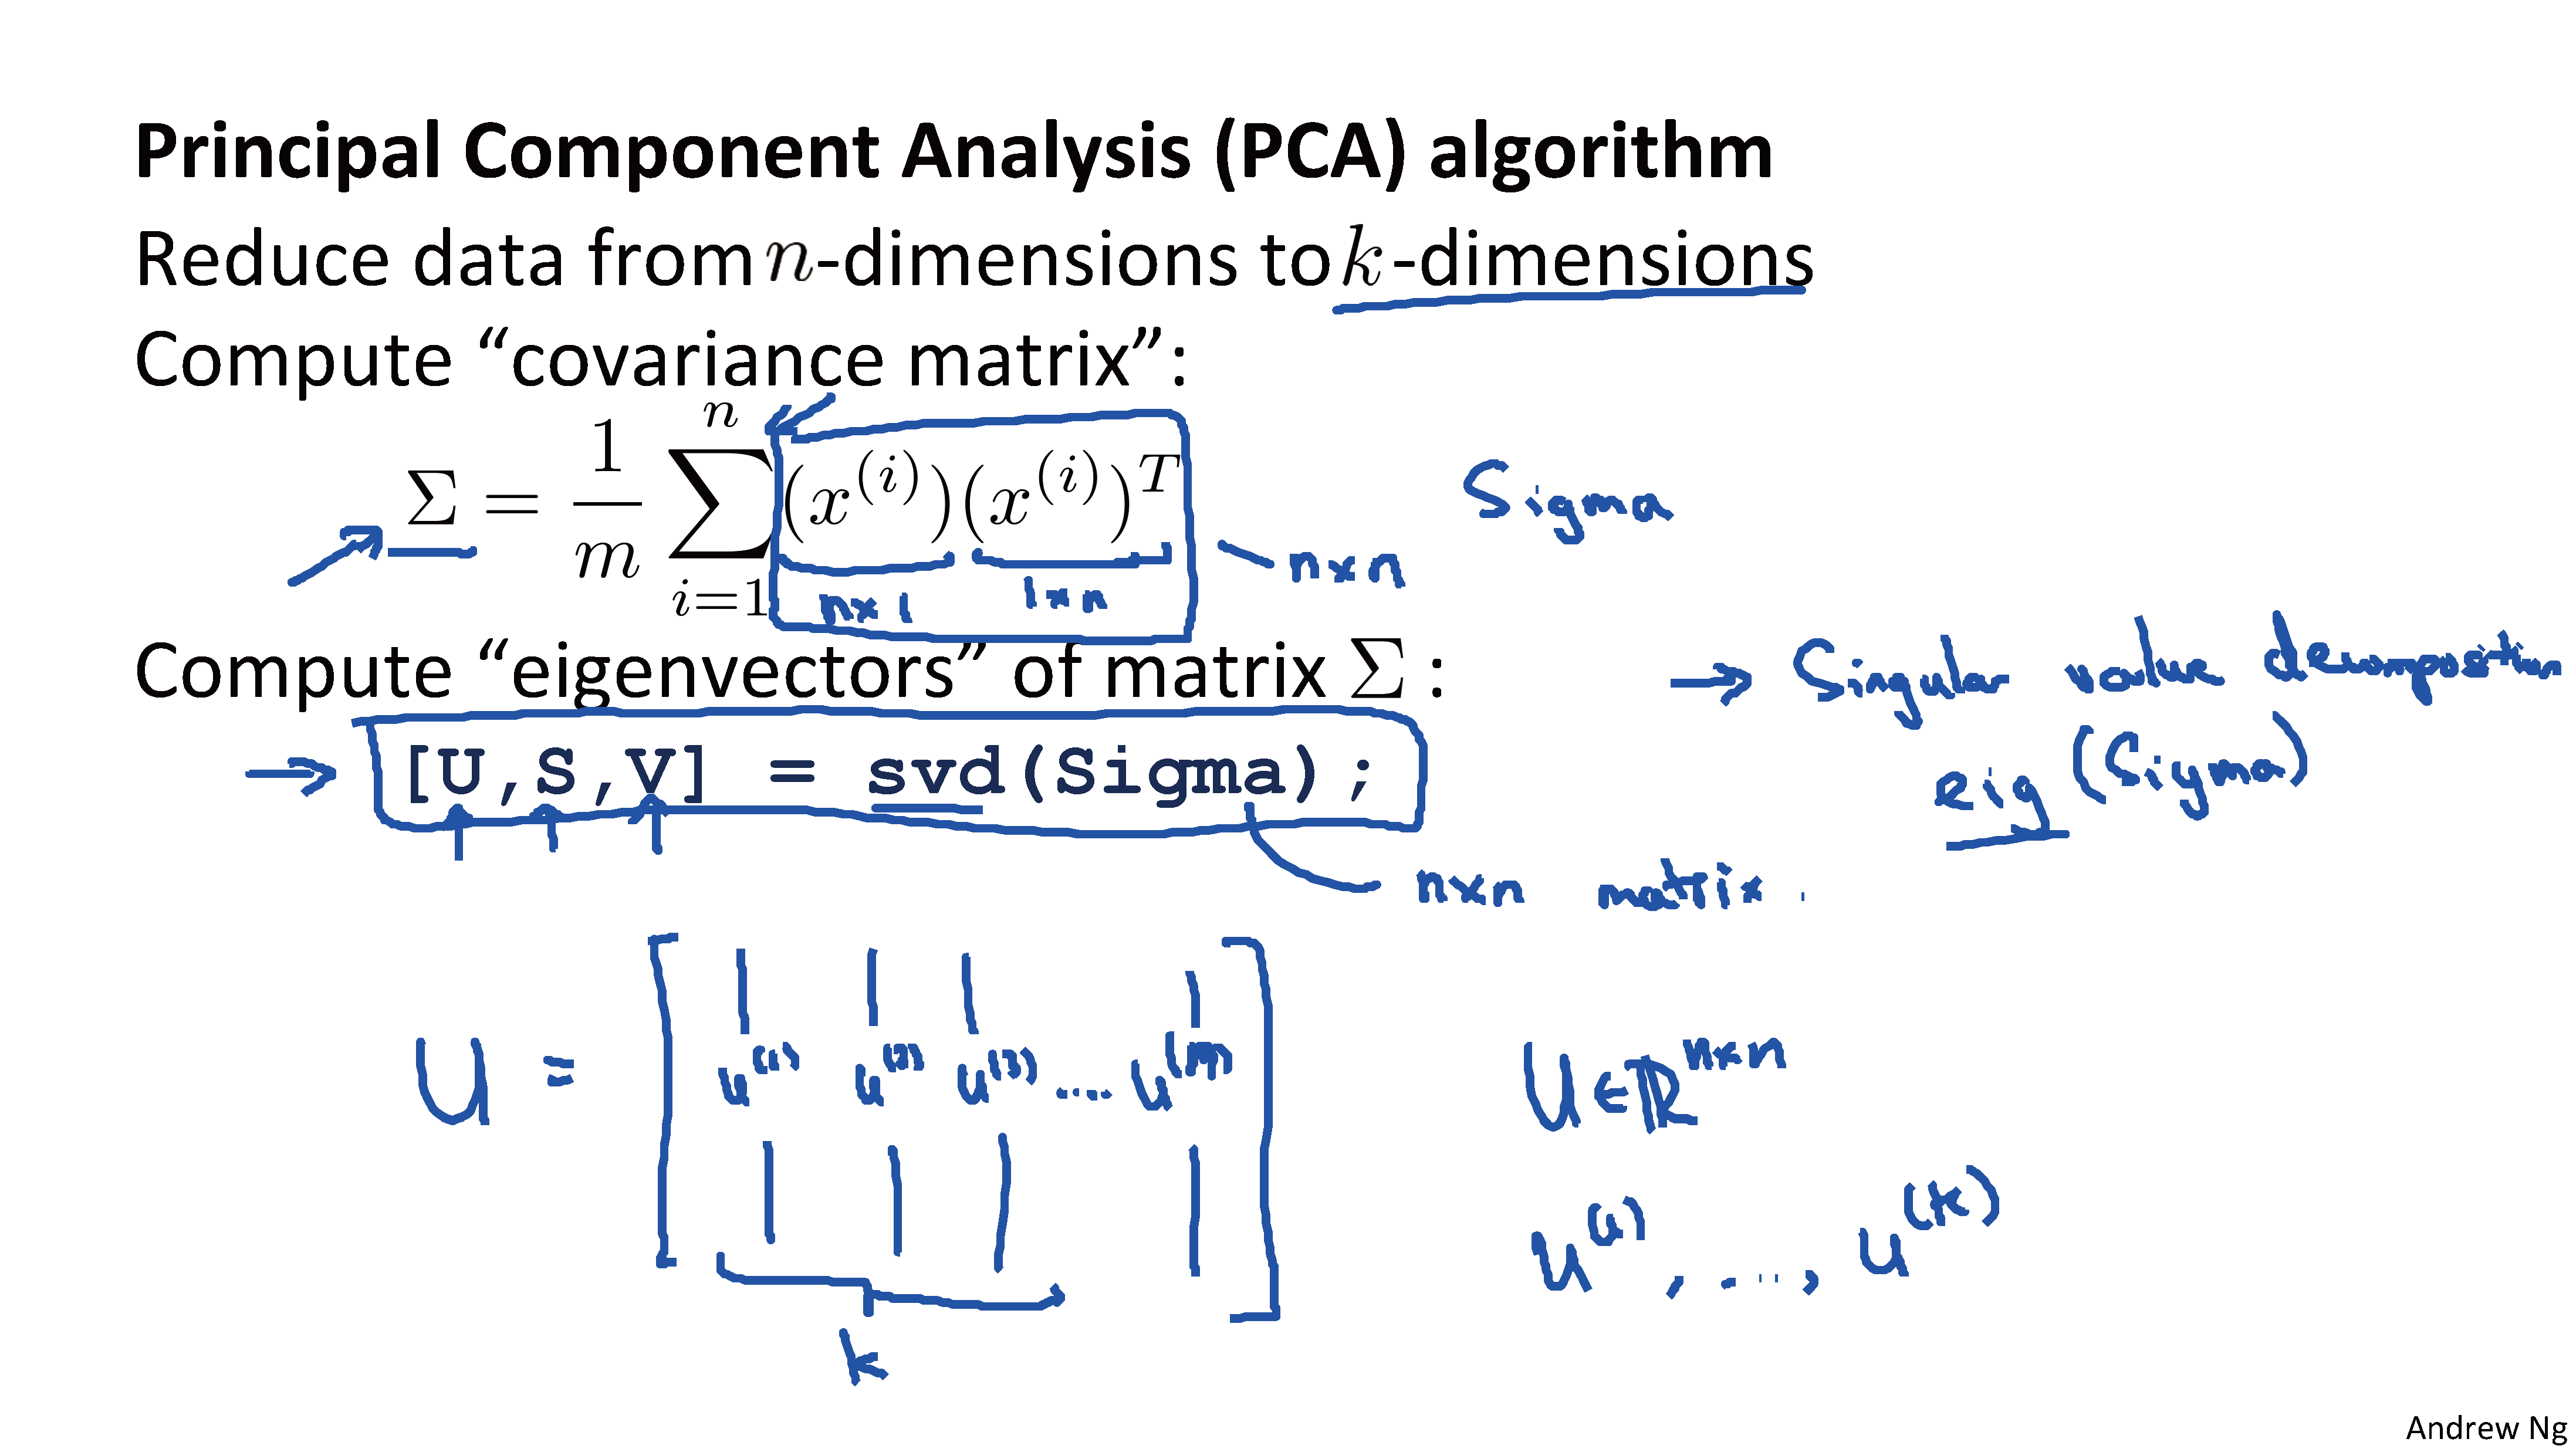
\includegraphics[width=0.95\linewidth]{pca3}
				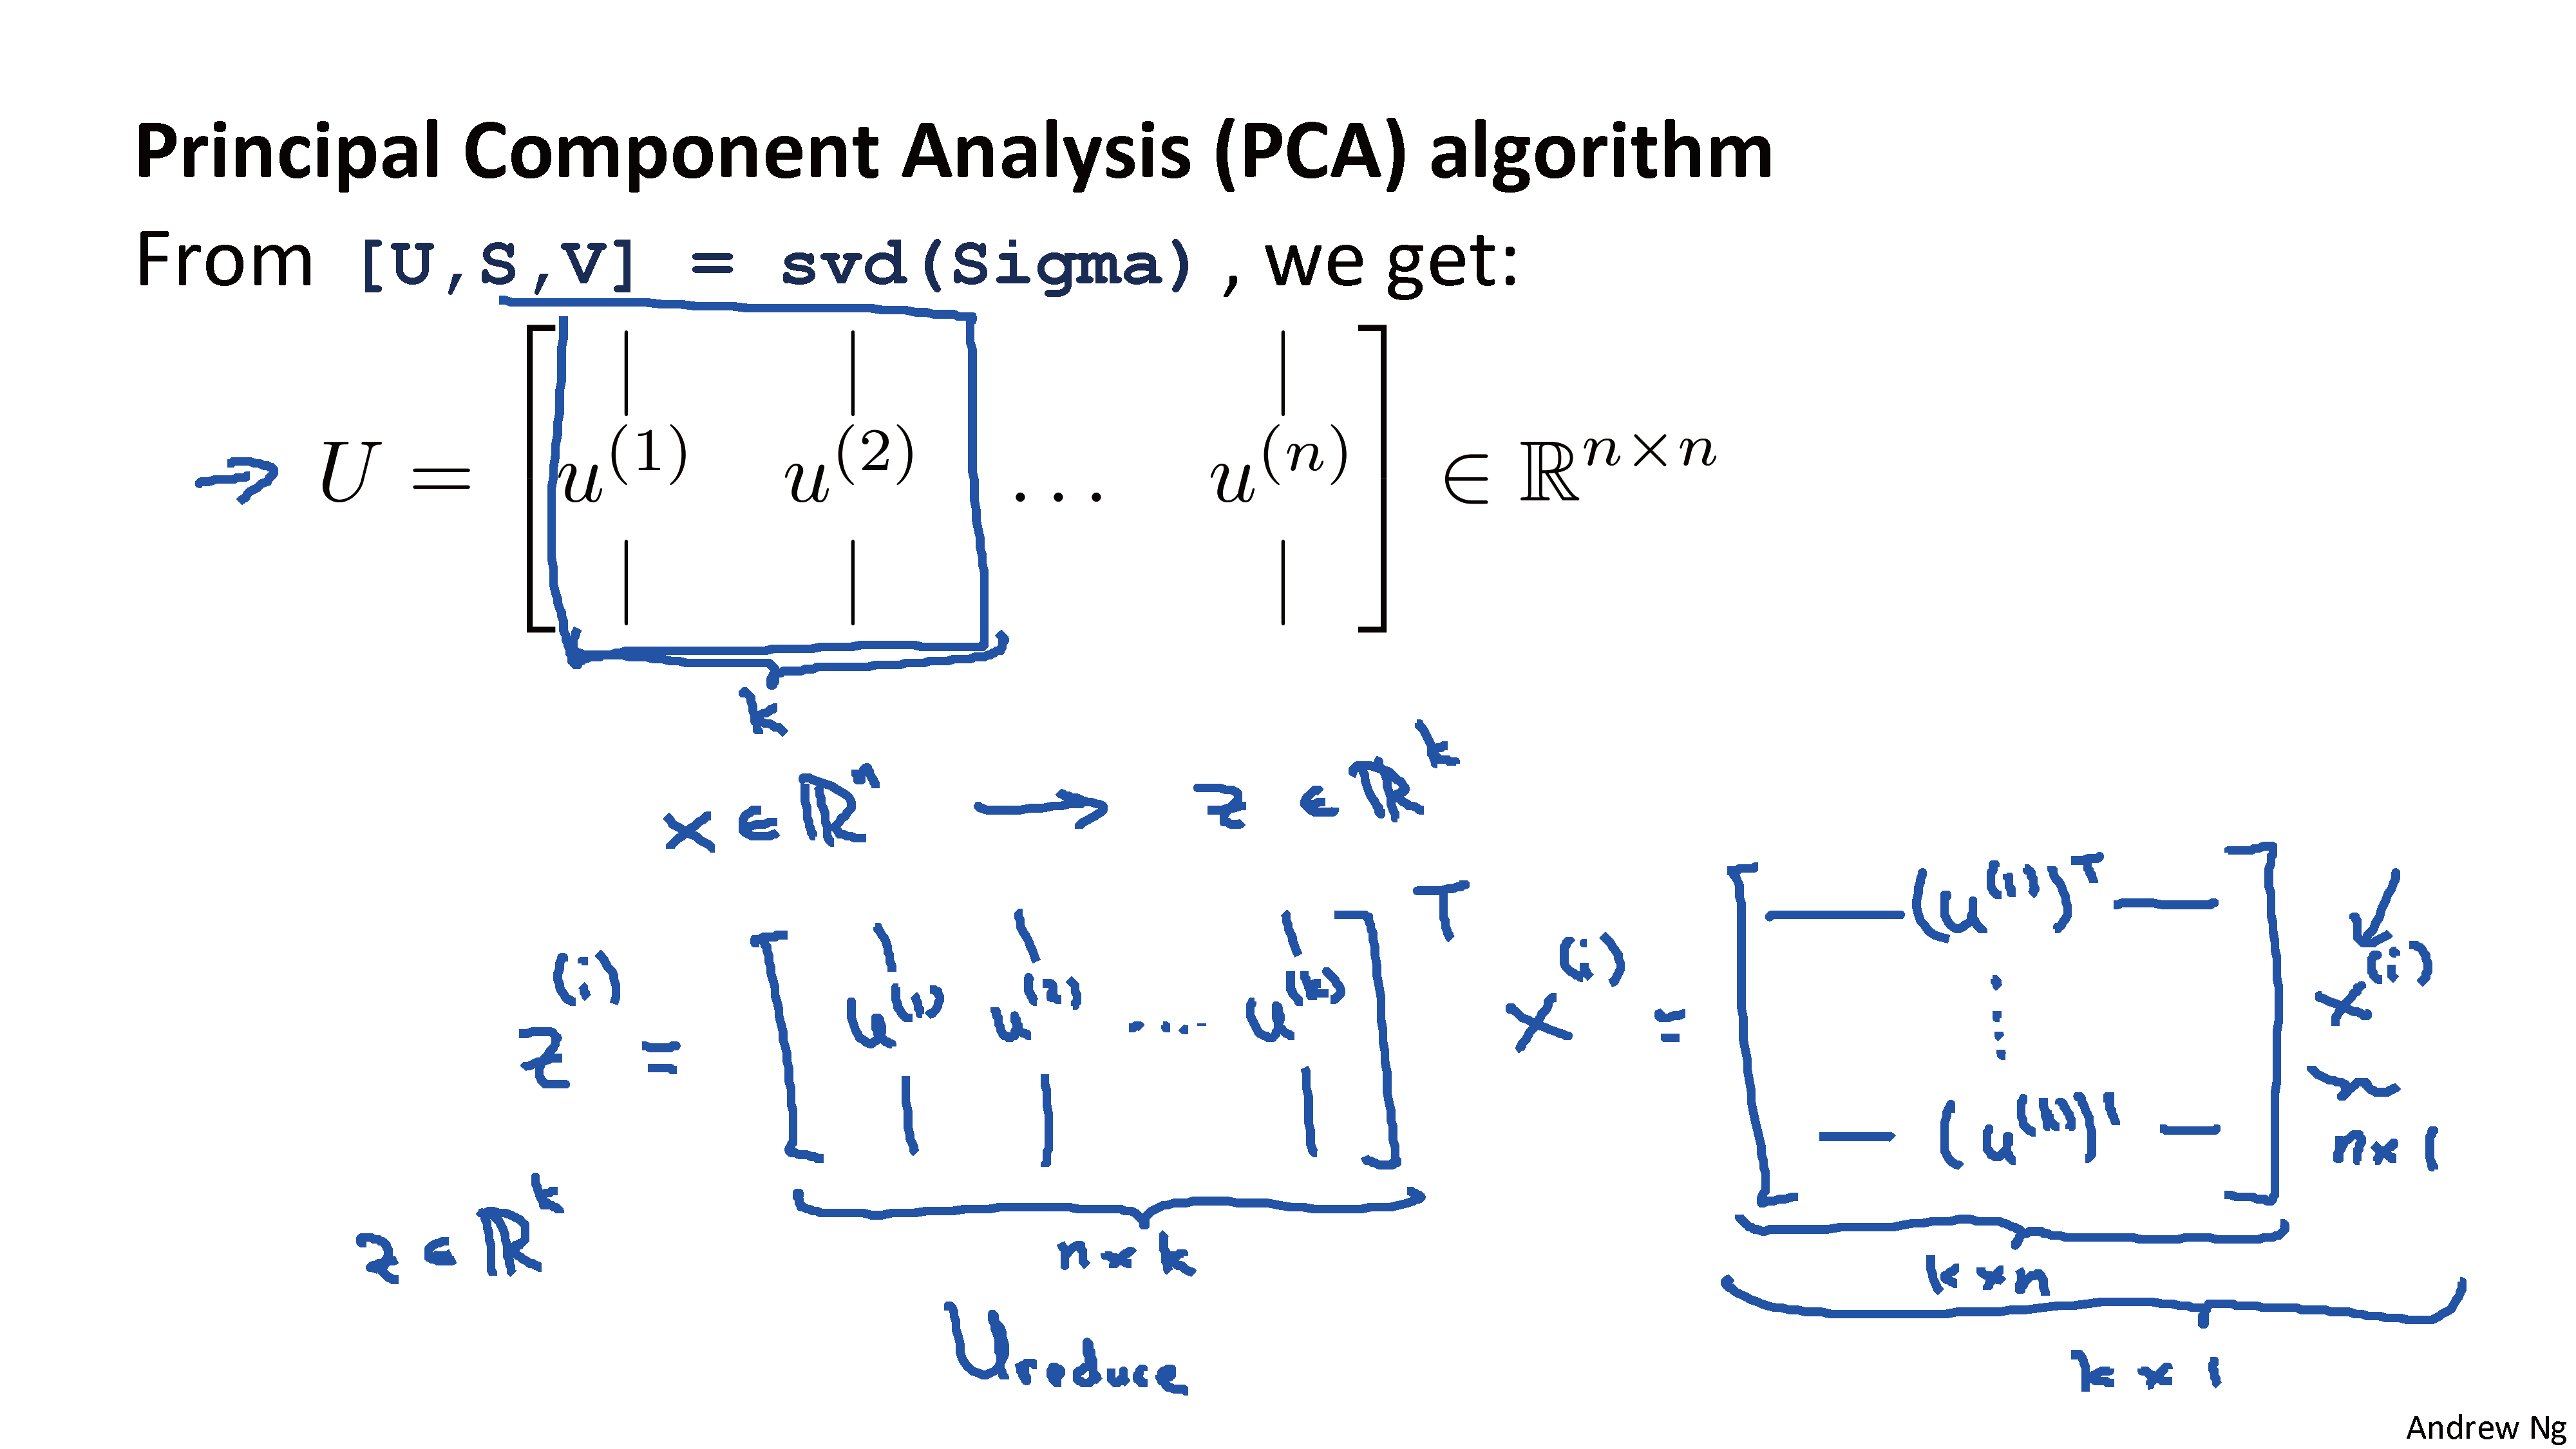
\includegraphics[width=0.95\linewidth]{pca4}
			\end{center}		
			$z = U_{redude} * X$
				\begin{itemize}
					\item Sensitive to scale: \textbf{Standardize before fitting!}
					\item Use $z$ in regression: Solve multicollinearity and increase degrees of freedom.
					\item Benefits: \textbf{Low dimension} and \textbf{No correlation of X}.
					\item Drawback: Hard to interpretate.
				\end{itemize}
				
		\section{Some True/False Questions}
			\begin{enumerate}
				\item A multiple linear regression model should only include explanatory variables that have a normal distribution. \textbf{FALSE}
				\item Adding an extra explanatory variable to a simple linear regression model \textbf{cannot} increase the significance, as measured by the t-test, for the explanatory	variable that is already in the model. \textbf{FALSE}
				\item  The main reason logistic regression is preferred to multiple linear regression for a categorical response with two categories is that the logistic regression model allows for the non-constant variance of the response. \textbf{FALSE}
				\item The multiple linear regression $\mu (Y | X ) = \beta_0 + \beta_1X_1 + \beta_2 X_2 + \beta_3X_3$ 	will have the same $R^2$ value as the multiple linear regression $\mu (Y | Z ) = \beta_0 + \beta_1Z_1 + \beta_2 Z_2 + \beta_3Z_3$ where $Z_1, Z_2, Z_3$ are the first three principal component variables of $X_1, X_2, X_3$ \textbf{TRUE}
				\item The bootstrap cannot be used for hypothesis testing. \text{FALSE}
				\item It is possible for the first three principal component variables ($Z_1,..., Z_3$) from a principal components analysis of ten variables ($X_1 ,..., X_10$) to explain 100\% of the total variation in the ten original variables $X_1 ,..., X_10$. \textbf{TRUE}
				\item The estimated mean response for the regression $\mu (Y | X ) = \beta_0 + \beta_1X_1 + \beta_2 X_2 + \beta_3(X_1\times X_2)$ corresponding to a particular set of explanatory variable values $X_1 =3, X_2 = 2$ is 15. Based on this information we
				would estimate that there is more than a 50\% chance that the response
				variable, given $X_1 =3, X_2 = 2$, would take on a value greater than 17. \textbf{FALSE}
				\item Modelling marital status (Single, Married, Divorced) as a categorical	explanatory variable in a Poisson log-linear regression model will require three parameters to be estimated, not including the intercept and other variables included in the model. \textbf{FALSE}
				\item A fitted linear regression model based on 500 observations returns
				$b_6=0.21, SE(b_5)=0.06$. You are given two 90\% confidence intervals (a)	(0.09,0.33) and (b) (0.13,0.42) that have been computed based on the fitted regression model. One of the intervals was computed using the bootstrap and another using the standard linear regression theory. Interval (b) (0.13,0.42) is	the confidence interval computed using the standard theory. \textbf{FALSE}
				\item There are 64 possible logistic regression models that can be fitted in a situation there are seven explanatory variables and we are only interested in models that contain these seven variables; that is, we are not including interactions terms, terms for curvature etc. \textbf{FALSE}
			\end{enumerate}
	\end{multicols}
\end{document}